% FlashCart project report — follows the TIET report template
% (US Letter, 12 pt, Computer Modern, right-aligned chapter heads, running header).
% Compile with pdfLaTeX / XeLaTeX (e.g. Overleaf) or `tectonic main.tex`.
\documentclass[12pt,letterpaper,twoside,openany]{report}

\usepackage[letterpaper,inner=1.5in,outer=1in,top=1.25in,bottom=1in,
            includehead,headheight=15pt,headsep=14pt]{geometry}
\usepackage{amsmath}
\usepackage{graphicx}
\usepackage{xcolor}
\usepackage{array}
\usepackage{enumitem}
\usepackage{rotating}
\usepackage{titlesec}
\usepackage{fancyhdr}
\usepackage[hidelinks,pagebackref=true]{hyperref}

\newcommand{\coursetitle}{UCS503 - Software Engineering}
\graphicspath{{figures/}}

% ---------- Chapter / section headings (template style) ----------
\titleformat{\chapter}[display]
  {\normalfont\bfseries\filleft}
  {\large\chaptertitlename\ \thechapter}{4pt}{\Huge}
  [{\vspace{2pt}\titlerule[0.4pt]}]
\titleformat{name=\chapter,numberless}[display]
  {\normalfont\bfseries\filleft}{}{0pt}{\Huge}
  [{\vspace{2pt}\titlerule[0.4pt]}]
\titlespacing*{\chapter}{0pt}{-18pt}{22pt}

% Let large figures sit on text pages (fewer half-empty float pages)
\renewcommand{\topfraction}{0.95}
\renewcommand{\bottomfraction}{0.95}
\renewcommand{\textfraction}{0.05}
\renewcommand{\floatpagefraction}{0.9}
\setcounter{topnumber}{3}
\setcounter{totalnumber}{4}
\titlespacing*{\section}{0pt}{3ex plus 1ex minus .2ex}{1.6ex plus .2ex}
\titlespacing*{\subsection}{0pt}{2.4ex plus 1ex minus .2ex}{1.2ex plus .2ex}

% ---------- Running header: page number + course title ----------
\pagestyle{fancy}
\fancyhf{}
\fancyhead[LE]{\thepage\quad\coursetitle}
\fancyhead[RO]{\coursetitle\quad\thepage}
\renewcommand{\headrulewidth}{0.4pt}
\fancypagestyle{plain}{\fancyhf{}\renewcommand{\headrulewidth}{0pt}}

% ---------- Lists, tables, citations ----------
\setlist{itemsep=2pt,topsep=4pt}
\setlength{\emergencystretch}{2em}
\renewcommand{\arraystretch}{1.15}
\renewcommand*{\backrefalt}[4]{\ifcase #1 \or (cit. on p.~#2)\else (cit. on pp.~#2)\fi}
\renewcommand*{\backrefsep}{, }
\renewcommand*{\backreftwosep}{, }
\renewcommand*{\backreflastsep}{, }

\begin{document}

% =====================================================================
% Title page
% =====================================================================
\begin{titlepage}
  \centering
  \vspace*{0.6in}
  {\large\bfseries \coursetitle\par}
  \vspace{0.7in}
  {\LARGE\bfseries FlashCart: Unified Mall Checkout\par}
  \vspace{6pt}
  Scan products across every showroom, pay once, get one GST invoice\par
  \vspace{1.1in}
  {\large\bfseries Submitted by:\par}
  \vspace{8pt}
  {\large
    \texttt{1024031127} Pranay Nagpal\par
    \texttt{1024031145} Suryansh Jain\par
    \texttt{1024031144} Srijan Tanwar\par}
  \vspace{10pt}
  Group: \texttt{3C82} BE Third Year, CSE\par
  \vspace{1.1in}
  {\large\bfseries Submitted to:\par}
  \vspace{6pt}
  Jhonsy Bansal\par
  \vfill
  {\large Mid-Semester Evaluation\par}
  \vspace{4pt}
  {\large\bfseries Computer Science and Engineering Department\par}
  \vspace{4pt}
  Thapar Institute of Engineering and Technology, Patiala\par
\end{titlepage}

\tableofcontents

% =====================================================================
\chapter{Introduction}
% =====================================================================

\section{Background and Context}
A modern Indian mall houses dozens of independent showrooms (apparel, electronics, food,
jewellery, beauty), and each runs its own billing counter. A shopper who buys a shirt,
earbuds and a coffee queues three times, pays three times and leaves with three bills, each
with its own GST calculation. \textbf{FlashCart} replaces these counters with one digital
checkout. The shopper signs in with a mobile number and scans the barcode on any product tag
with the phone camera. Every item from every showroom lands in one \emph{unified bag}, which
is paid once (UPI or card through Razorpay, or cash at a central desk) for a single GST
invoice.

\subsection{Problem Statement}
Multi-showroom retail suffers from repeated queues and payments per store, fragmented
receipts that are hard to audit for GST, manual cash handling with change errors and no
reliable end-of-day drawer total, and carts that are lost when a device changes. The project
builds a web-based unified checkout that removes these problems without new hardware in the
showrooms, using the EAN-13 barcodes already printed on retail tags.

\section{Project Objectives}
\begin{enumerate}[leftmargin=*]
  \item \textbf{Objective 1:} Phone-number sign-in and camera scanning of EAN-13 / UPC /
        Code 128 barcodes, adding an item to the bag in under one second.
  \item \textbf{Objective 2:} An exact multi-slab GST bill (5\%, 12\%, 18\%) across all
        showrooms, including tags whose MRP already includes GST.
  \item \textbf{Objective 3:} One payment: Razorpay (UPI / card) with server-side HMAC-SHA256
        verification, or cash at a desk.
  \item \textbf{Objective 4:} An email-and-password cash desk that shows the change to return
        and the cash left in the drawer at day end.
  \item \textbf{Objective 5:} Persist all data in a database and cover the business rules
        with automated tests, delivered in three iterations (Section~\ref{sec:sdlc}).
\end{enumerate}

% =====================================================================
\chapter{Methodology and Design}
% =====================================================================

\section{System Architecture}

\subsection{High-Level Design}
FlashCart follows a three-tier client--server architecture
(Figure~\ref{fig:arch}). Two single-page applications run in the browser: the
\emph{customer app} on the shopper's phone, and the \emph{cash desk} on a counter tablet or
laptop. Both talk JSON over HTTPS to one Express REST API, and every protected call carries a
signed bearer token. The API owns all business rules: pricing, stock, payment
verification and cash accounting. Clients never send amounts, they only send intents.
Durable data lives in an SQLite database, while short-lived carts and gateway orders are kept
in memory. Online payments go through Razorpay~\cite{razorpay}.

\begin{figure}[!htb]
  \centering
  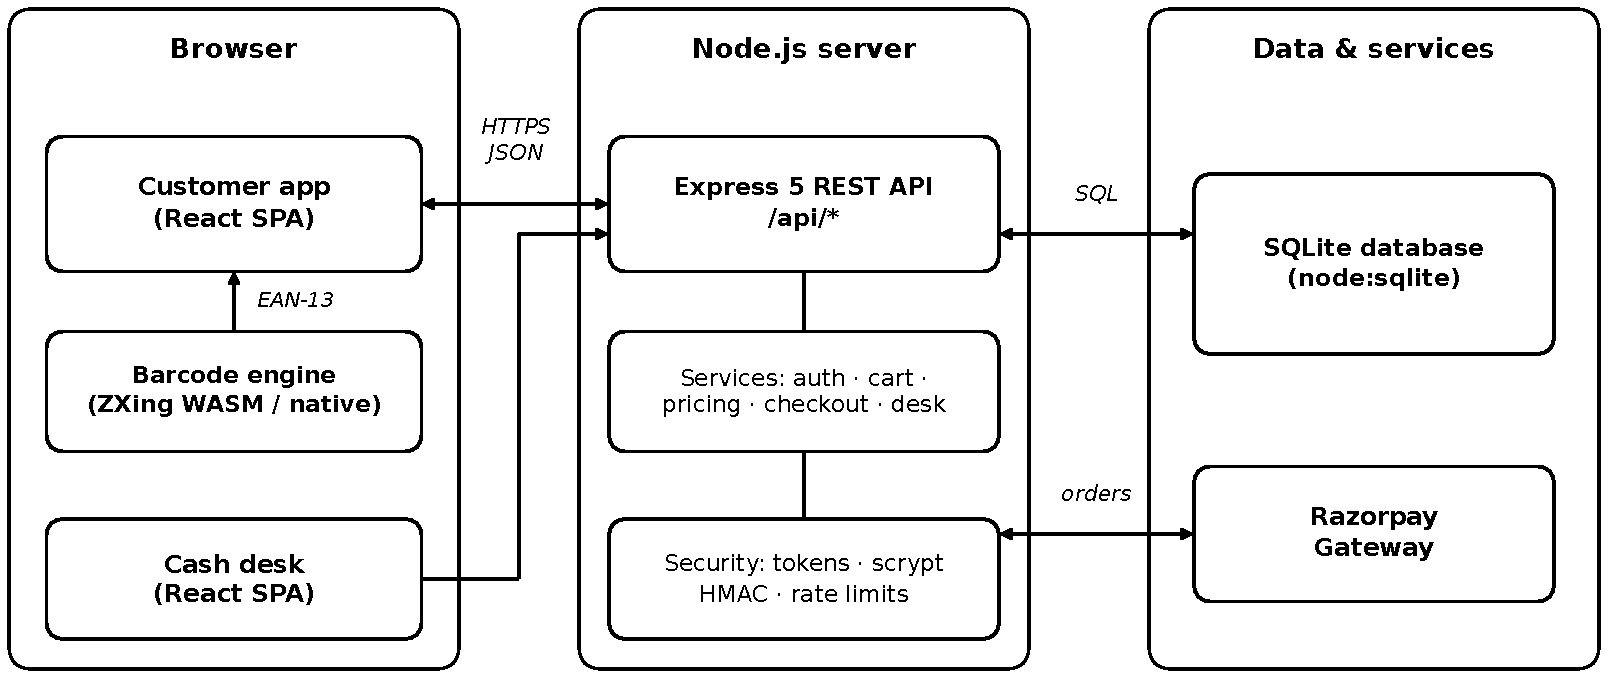
\includegraphics[width=\textwidth]{architecture}
  \caption{High-level three-tier architecture of FlashCart}
  \label{fig:arch}
\end{figure}

\subsection{Technical Stack}
\begin{itemize}[leftmargin=*]
  \item \textbf{Framework/Language:} JavaScript (ES2022). React~19 with Vite~8 for the
        two web apps~\cite{react,vite}; Node.js~22+ with Express~5 for the REST
        API~\cite{express}.
  \item \textbf{Database:} SQLite through Node's built-in \texttt{node:sqlite}
        module~\cite{nodesqlite}: one file, no separate database server.
  \item \textbf{Tools:} Git and GitHub, npm, Vite HTTPS dev server for testing on phones,
        Razorpay test-mode dashboard, oxlint, and the built-in \texttt{node:test} runner.
  \item \textbf{Libraries:} Tailwind CSS~4, Lucide icons and Axios for the UI; ZXing-C++
        compiled to WebAssembly for barcode reading~\cite{zxing,shapedetect}; JsBarcode
        for bill barcodes; the Razorpay Node SDK, uuid and dotenv on the server.
\end{itemize}

\section{Implementation Details}

\subsection{Module 1: Customer App and Barcode Scanning}
After a phone-number sign-in the customer lands on a home screen (bag total, showrooms,
recent receipts). The camera opens only on the \emph{Scan} screen. It uses the rear camera
at 1920$\times$1080 and decodes a wide central band every 90\,ms, plus the full frame every
fourth pass for tags held off-centre. Decoding uses the native \texttt{BarcodeDetector}
where available (Chrome)~\cite{shapedetect}, and otherwise ZXing-C++ compiled to
WebAssembly~\cite{zxing}, which the app serves itself and loads only when the scanner opens.
Only linear formats are enabled (EAN-13/8~\cite{gs1}, UPC, Code 128/39, ITF), so a QR code on
the same tag is never picked up. Repeat reads within 2.2\,s are ignored. A beep, a haptic
tick and an \emph{Undo} action confirm each scan, and manual entry and catalog search
work without a camera.

\subsection{Module 2: GST Pricing and Unified Checkout}
All arithmetic uses integer paise. For GST-exclusive prices, tax is
$\mathrm{round}(\text{subtotal}\times\text{rate})$. Real tags print an MRP that
\emph{includes} tax, so the line total is exactly $\text{MRP}\times\text{qty}$ and the taxable
value is $\text{MRP}\div(1+\text{rate})$. For example, a Rs.~2999 polo bills as Rs.~2541.53
taxable + Rs.~457.47 GST. Tax is summed per slab, split into CGST and SGST, and rounded to
the rupee, and invoice numbers run per financial year (\texttt{FC/2627/000001}). For online
payment the server prices the bag, creates the Razorpay order, and verifies
$\text{HMAC-SHA256}(\textit{order\_id}\,|\,\textit{payment\_id})$ in constant
time~\cite{hmac,razorpay} before saving the invoice and reducing stock in one SQLite
transaction. Replayed callbacks return the same receipt.

\subsection{Module 3: Cash Desk and End-of-Day Drawer}
Choosing cash issues a \emph{pending} invoice with a Code~128 bill barcode. The cashier
(signed in by email and password) records the opening cash, then finds the bill by scanning
it or typing the customer's phone number. Entering the cash received shows the
\emph{change to return} with a note split: Rs.~5000 for a Rs.~3894 bill gives Rs.~1106 as
$2\times500+100+5+1$. Short payments are rejected. The drawer panel shows
\emph{opening cash + cash sales}. At closing, the counted cash is compared with that figure
to report any overage or shortage, and a printable day report is produced. The customer's
receipt turns \emph{Paid} as soon as the cash is recorded.

\subsection{Module 4: Authentication and Database}
Customers sign in with a 10-digit mobile number; cashiers with an email and a salted scrypt
password hash~\cite{scrypt}. Sessions are HMAC-signed tokens (30 days for customers, 12 hours
for cashiers), role guards keep each role in its own API area, and login endpoints are
rate-limited. Table~\ref{tab:db} lists the schema.

\begin{table}[!htb]
  \centering
  \small
  \begin{tabular}{|l|p{0.62\textwidth}|}
    \hline
    \textbf{Table} & \textbf{Key columns} \\ \hline
    customers    & phone (unique), created\_at, last\_login\_at \\ \hline
    cashiers     & email (unique), name, password\_hash, active \\ \hline
    products     & barcode (EAN-13), name, cost, mrp, gst, type, hsn, showroom, stock \\ \hline
    transactions & invoice no., customer, grand total, method, status, cash received, change \\ \hline
    cash\_shifts & cashier, opening cash, opened/closed at, counted cash \\ \hline
  \end{tabular}
  \caption{SQLite database schema}
  \label{tab:db}
\end{table}

\section{Software Development Life Cycle}\label{sec:sdlc}
We followed an \textbf{iterative and incremental (agile)} SDLC~\cite{sommerville}
(Figure~\ref{fig:sdlc}). Each iteration went through requirements, design, build, test, demo
and review, and the review feedback set the next scope: iteration~1 (weeks 1--6) built the MVP,
iteration~2 (weeks 7--8) added sign-in, SQLite and the cash desk, and iteration~3 (weeks 9--10)
added the barcode engine, real products and MRP pricing.

\begin{figure}[!htb]
  \centering
  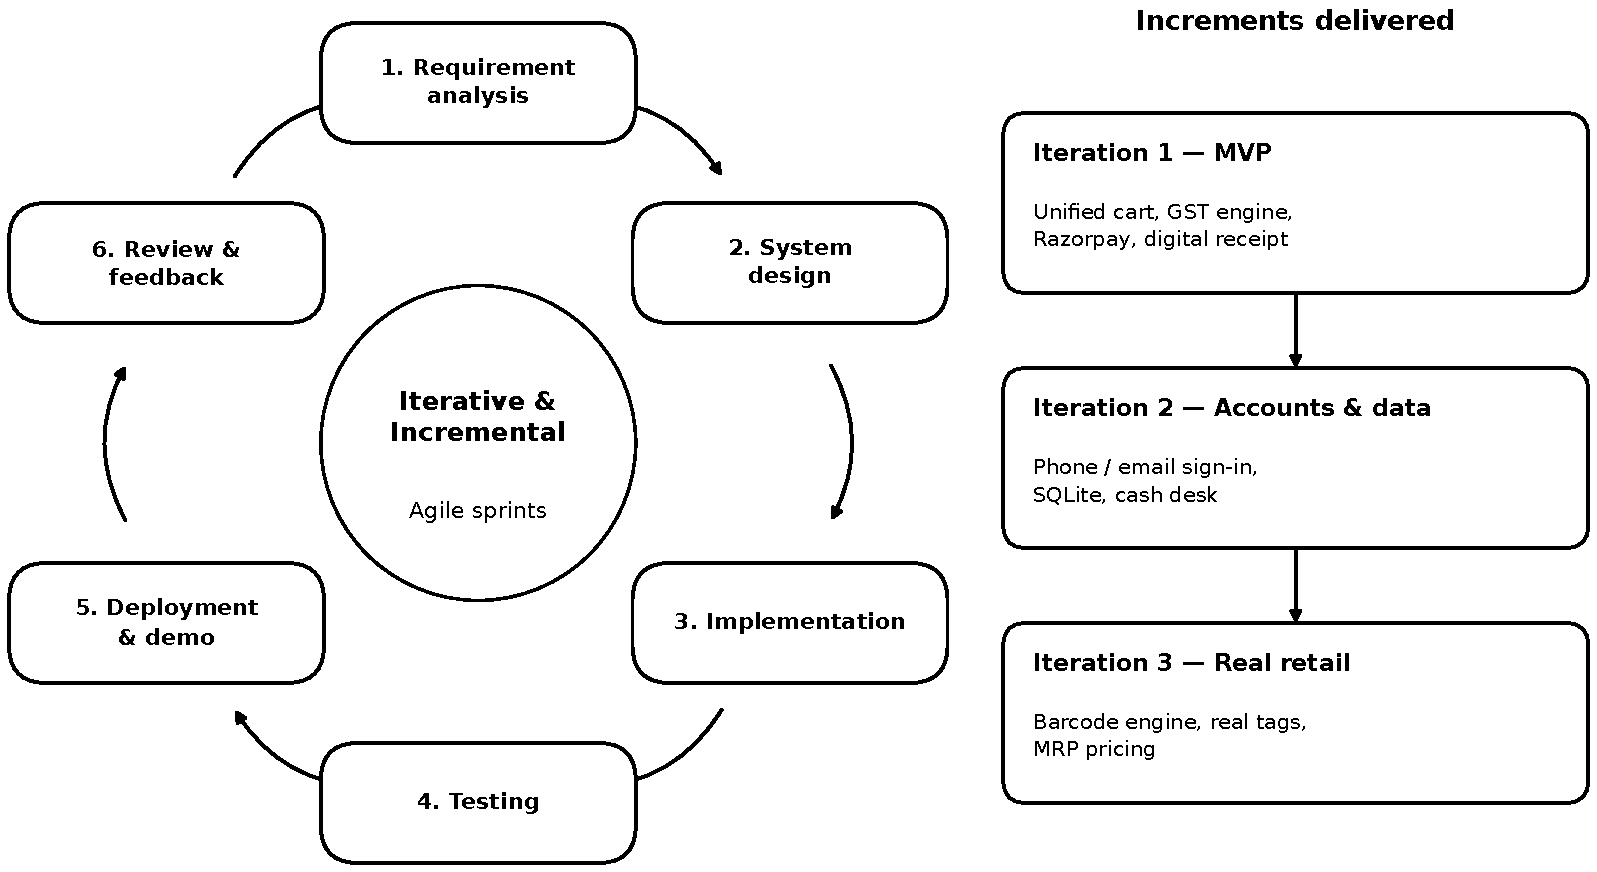
\includegraphics[width=\textwidth]{sdlc}
  \caption{Iterative and incremental SDLC with the three delivered increments}
  \label{fig:sdlc}
\end{figure}

\section{UML Diagrams}
The design is modelled with four UML~\cite{fowler} views: use case, sequence, activity
and class diagrams.

\subsection{Use Case Diagram}
Figure~\ref{fig:usecase} shows two primary actors and one external system. The
\emph{Customer} signs in, scans or browses (both include \emph{Add item to bag}), manages the
bag and checks out. \emph{Pay online} and \emph{Pay cash at the desk} extend Checkout, and
online payment always includes signature verification with \emph{Razorpay}. The
\emph{Cashier} signs in, starts the day, finds bills, collects cash and closes the day.

\begin{figure}[!htb]
  \centering
  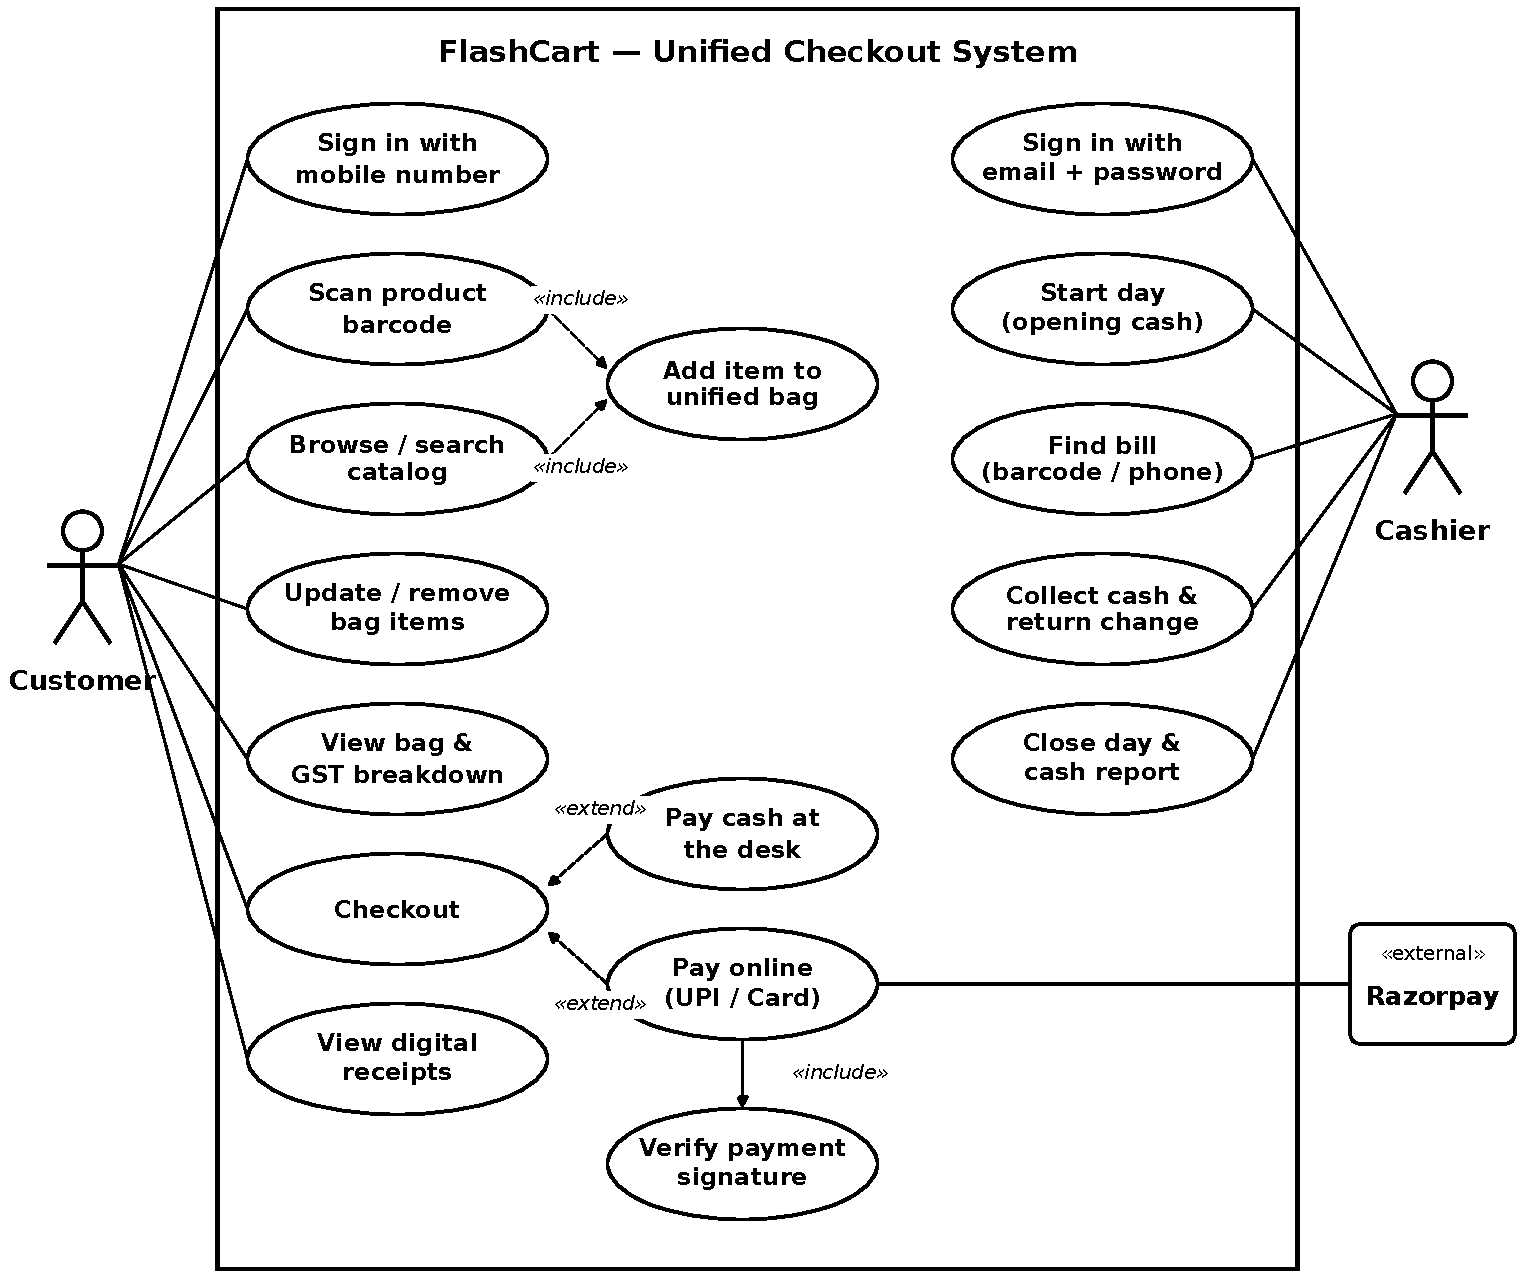
\includegraphics[width=0.95\textwidth]{use_case}
  \caption{Use case diagram}
  \label{fig:usecase}
\end{figure}

\subsection{UML Sequence Diagram}
Figure~\ref{fig:sequence} traces an online payment across the customer, the React frontend,
the Express backend, the SQLite database and Razorpay. The amount is computed only on the
server (steps 3--5), and no invoice is written unless the signature check in step~12
succeeds. The \texttt{alt} fragment shows both outcomes.

\begin{figure}[!htb]
  \centering
  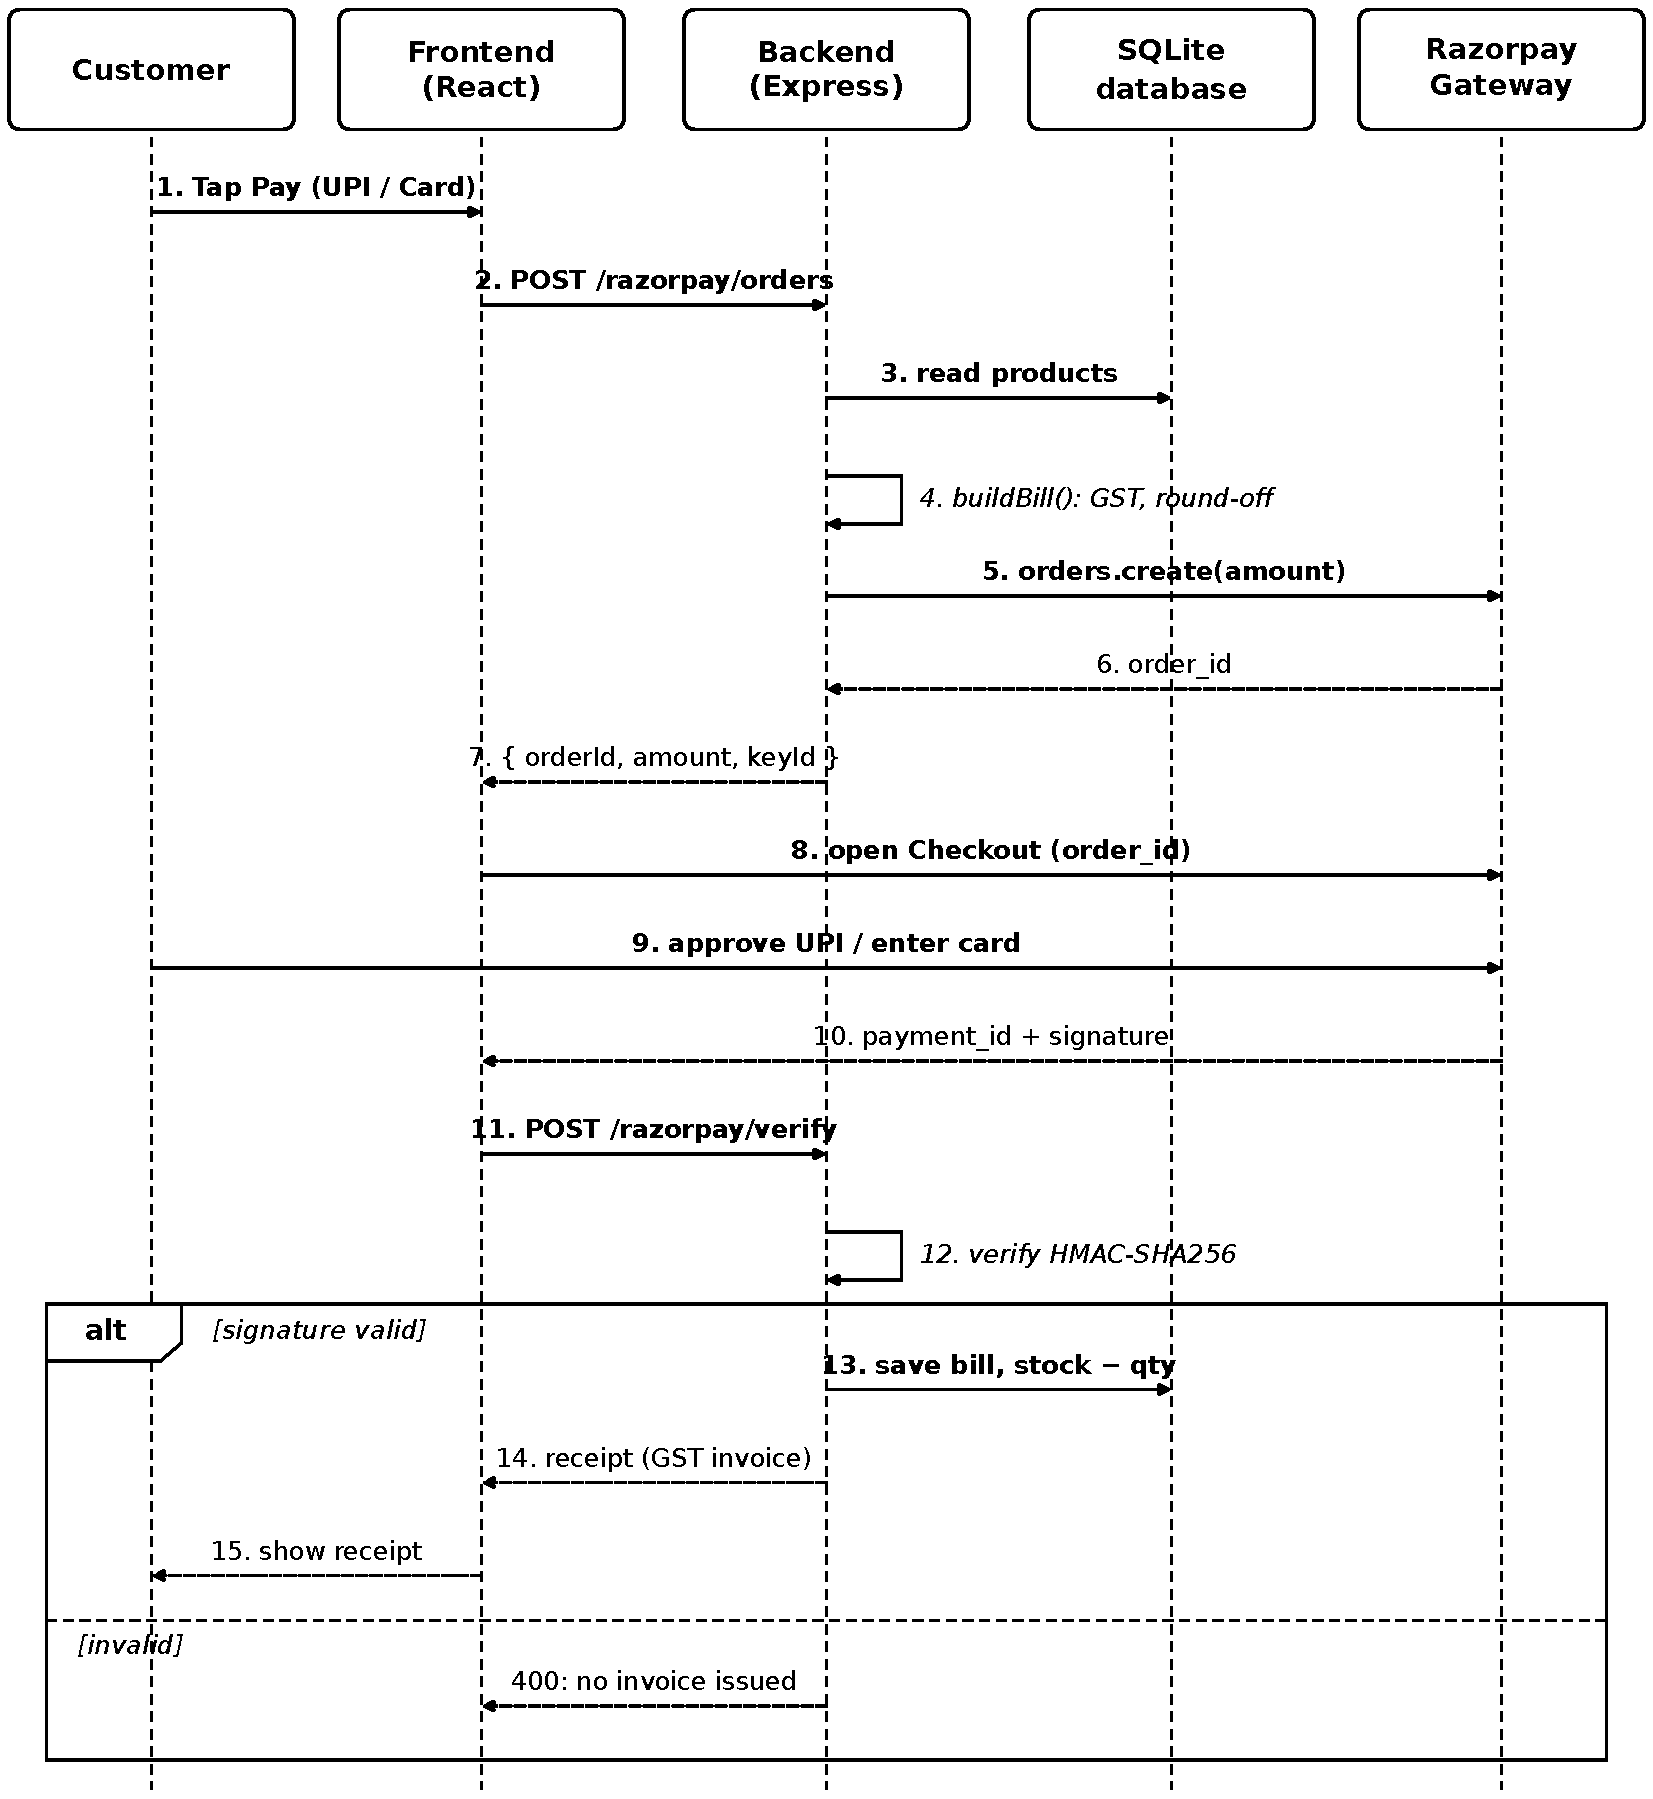
\includegraphics[width=\textwidth]{sequence}
  \caption{UML sequence diagram: checkout and Razorpay payment flow}
  \label{fig:sequence}
\end{figure}

\subsection{Activity Diagram}
Figure~\ref{fig:activity} models the customer's checkout. A scan loops back on an invalid
or out-of-stock code. The bag grows until the customer proceeds. The flow then forks
on the payment method: online payments retry until the signature verifies, while cash bills
wait for the cashier. Both paths merge at a single \emph{Paid} receipt.

\begin{figure}[!htb]
  \centering
  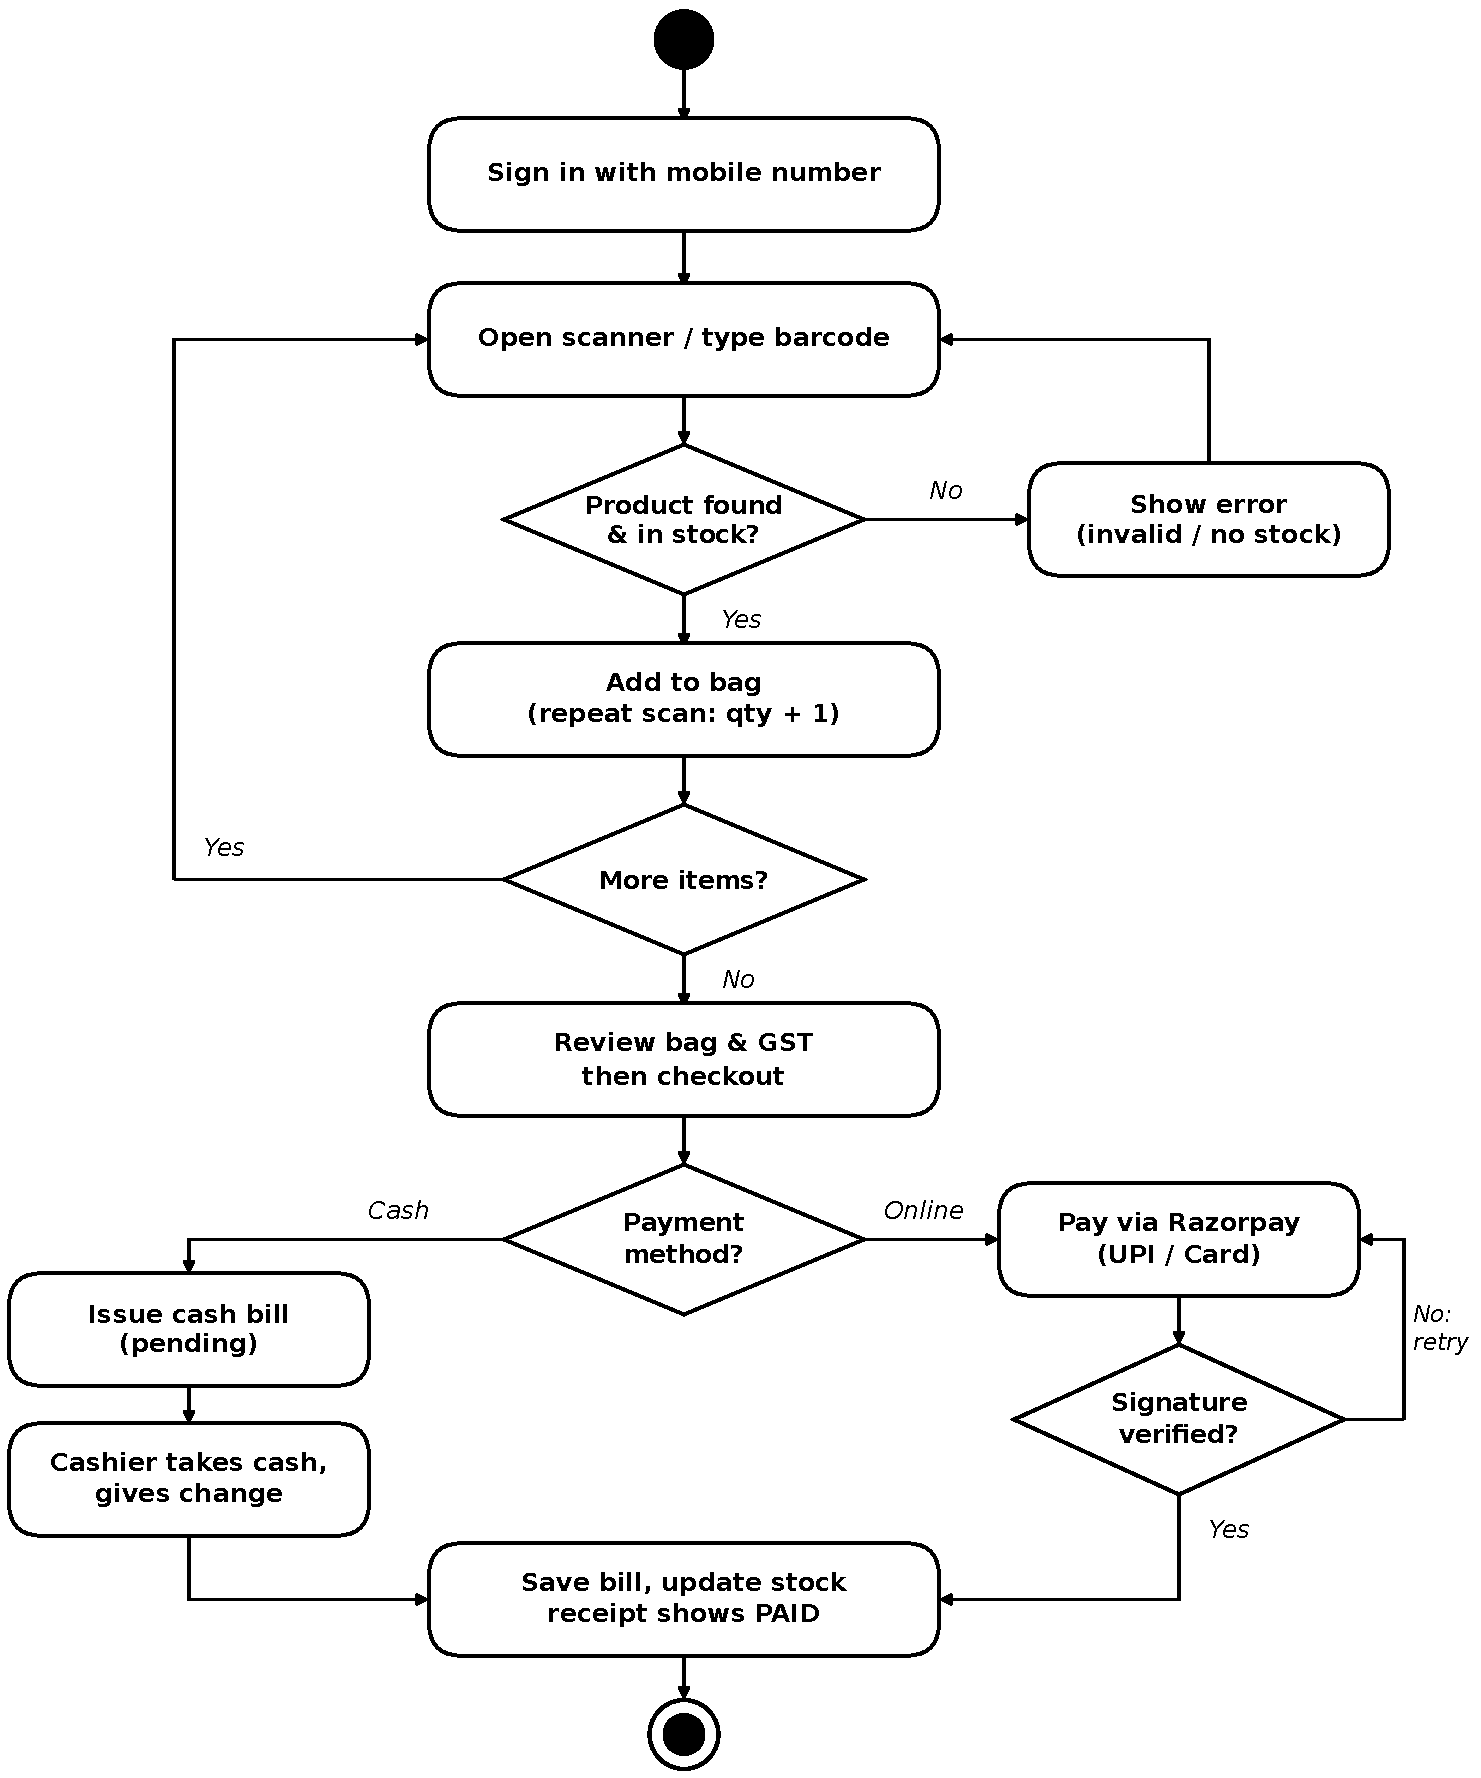
\includegraphics[width=0.86\textwidth]{activity}
  \caption{Activity diagram: customer checkout flow}
  \label{fig:activity}
\end{figure}

\subsection{Class Diagram}
Figure~\ref{fig:class} is the domain model. A \emph{Customer} owns shopping sessions; a
session is composed of \emph{CartLine}s that refer to \emph{Product}s, and checks out as
at most one \emph{Transaction} (bill). Cash bills are collected within a \emph{CashShift}
opened by a \emph{Cashier}. Transactions use the stateless \emph{PricingEngine} and
\emph{PaymentGateway} services.

\begin{sidewaysfigure}
  \centering
  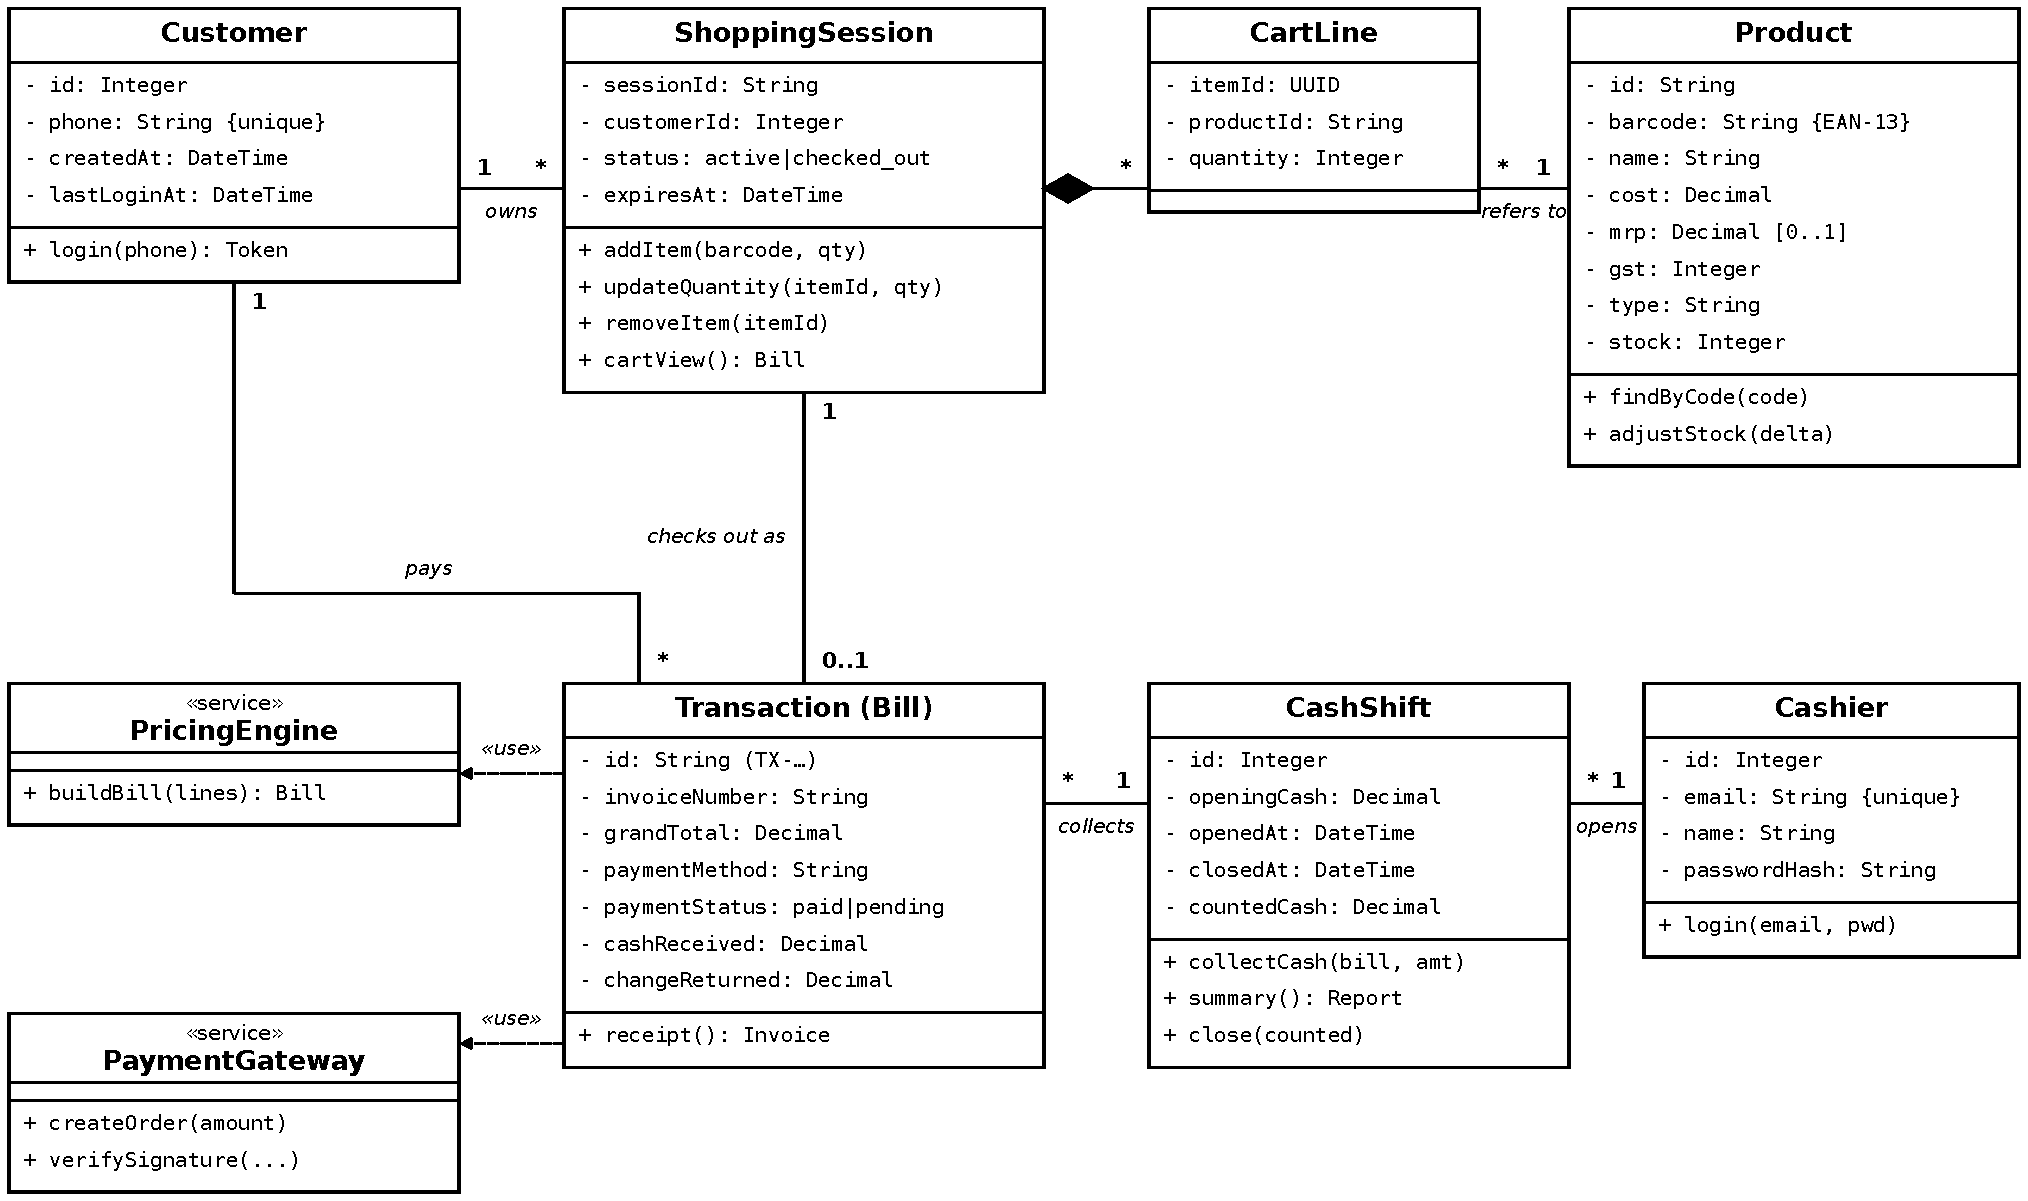
\includegraphics[width=\textheight]{class}
  \caption{Class diagram: FlashCart domain model}
  \label{fig:class}
\end{sidewaysfigure}

% =====================================================================
\chapter{Results and Evaluation}
% =====================================================================

\section{Testing Methodology}
\begin{itemize}[leftmargin=*]
  \item \textbf{Unit Testing:} the GST engine: slab totals, CGST/SGST split, round-off and
        MRP back-calculation.
  \item \textbf{Integration Testing:} 17 automated API tests (\texttt{node:test}) on the real
        Express app with an in-memory SQLite database: roles, cart, stock limits, Razorpay
        signatures (forged rejected, replays idempotent) and a full cash-desk day.
  \item \textbf{Performance Testing:} scripted load (90 customers $\times$ 3 scans, 90 cash
        bills, 50 collections) and barcode decode timing on photos of real tags.
  \item \textbf{User Testing:} browser end-to-end runs, a Razorpay test checkout, and real
        tags (Puma polo, Mufti shirt, JPG parfum).
\end{itemize}

\section{Performance Metrics}

\begin{table}[!htb]
  \centering
  \small
  \begin{tabular}{|l|r|r|}
    \hline
    \textbf{Metric} & \textbf{Target} & \textbf{Achieved} \\ \hline
    Add-to-bag API latency (p95) & $<$ 100 ms & 0.45 ms \\ \hline
    Cash collection API latency (p95) & $<$ 100 ms & 1.13 ms \\ \hline
    Barcode decode per frame (WebAssembly) & $<$ 100 ms & 25--35 ms \\ \hline
    Real product tags decoded & 3 / 3 & 3 / 3 \\ \hline
    Bill total vs.\ printed MRP & exact & exact \\ \hline
    Automated tests passing & 100\% & 17 / 17 \\ \hline
    Initial JavaScript download (gzip) & $<$ 150 KB & 77.8 KB \\ \hline
  \end{tabular}
  \caption{Performance results summary (Apple M4, server-side latencies)}
  \label{tab:results}
\end{table}

\section{Analysis}
\begin{itemize}[leftmargin=*]
  \item \textbf{Objectives:} all five met. Scanning, which \emph{failed} in the mid-term MVP,
        now reads real retail tags, and real-tag bills equal the printed MRP.
  \item \textbf{Challenges and fixes:} the MVP's QR-oriented scanner missed 1D barcodes, so we
        moved to native / ZXing-C++ decoding. MRP tags include GST, so we added tax-inclusive
        pricing. Data was lost on restart, so we added SQLite.
\end{itemize}

% =====================================================================
\chapter{Conclusion}
% =====================================================================

\section{Summary of Work}
FlashCart delivers a working unified checkout for multi-showroom retail. Customers sign in
with a phone number, scan real barcodes into one bag and pay once by UPI, card or cash.
Cashiers get a focused cash desk with change calculation and a reconciled end-of-day total.
Data is persisted in SQLite, and the rules are covered by automated tests.

\section{Key Findings}
\begin{itemize}[leftmargin=*]
  \item \textbf{Finding 1:} the EAN-13 codes already on tags are enough to run checkout.
  \item \textbf{Finding 2:} pricing must accept MRP-inclusive tags.
  \item \textbf{Finding 3:} server-side pricing and signature checks keep the client untrusted.
\end{itemize}

\section{Future Work and Recommendations}
\begin{enumerate}[leftmargin=*]
  \item \textbf{Inventory management:} a per-showroom inventory module for goods received,
        transfers and adjustments. It would add low-stock alerts and reorder suggestions,
        batch and expiry tracking for food, and an admin panel to add products (barcode, cost,
        MRP, GST, type), plus sales analytics and a daily stock reconciliation.
  \item \textbf{Hardware smart cart:} a physical trolley with a mounted barcode scanner (or
        RFID reader), a Raspberry Pi / ESP32 and a touchscreen, joined to the same FlashCart
        session over Wi-Fi. A load cell (HX711) would check the measured weight against the
        scanned items to catch unscanned goods, and the customer could pay on the cart itself.
  \item \textbf{Security:} SMS OTP for phone sign-in, Razorpay webhooks, returns and refunds.
  \item \textbf{Scale:} PostgreSQL, cloud deployment and a pilot in one mall wing.
\end{enumerate}

\section{Final Remarks}
The project covered the full software engineering cycle, from real retail requirements and UML
models to tested increments. Letting demo feedback reshape the design made FlashCart simpler
and more useful.

% =====================================================================
\begin{thebibliography}{Som16}
\addcontentsline{toc}{chapter}{Bibliography}
\raggedright

\bibitem[Exp25]{express} OpenJS Foundation. \emph{Express 5 API reference}.
  \url{https://expressjs.com/en/5x/api.html}. 2025.

\bibitem[Fow03]{fowler} M. Fowler. \emph{UML Distilled: A Brief Guide to the Standard
  Object Modeling Language}. 3rd ed. Addison-Wesley, 2003.

\bibitem[GS124]{gs1} GS1. \emph{GS1 General Specifications} (EAN/UPC barcodes).
  \url{https://www.gs1.org/standards/barcodes-epcrfid-id-keys/gs1-general-specifications}. 2024.

\bibitem[KBC97]{hmac} H. Krawczyk, M. Bellare, and R. Canetti. \emph{HMAC: Keyed-Hashing
  for Message Authentication}. RFC 2104. IETF, 1997.

\bibitem[Nod25]{nodesqlite} OpenJS Foundation. \emph{Node.js documentation:
  \texttt{node:sqlite}}. \url{https://nodejs.org/api/sqlite.html}. 2025.

\bibitem[PJ16]{scrypt} C. Percival and S. Josefsson. \emph{The scrypt Password-Based Key
  Derivation Function}. RFC 7914. IETF, 2016.

\bibitem[Raz25]{razorpay} Razorpay. \emph{Payment Gateway: Integration Steps and Payment
  Signature Verification}. \url{https://razorpay.com/docs/payments/payment-gateway/}. 2025.

\bibitem[Rea25]{react} Meta Open Source. \emph{React documentation}.
  \url{https://react.dev}. 2025.

\bibitem[Som16]{sommerville} I. Sommerville. \emph{Software Engineering}. 10th ed.
  Pearson, 2016.

\bibitem[Vit25]{vite} Vite team. \emph{Vite: Next Generation Frontend Tooling}.
  \url{https://vite.dev}. 2025.

\bibitem[WIC24]{shapedetect} W3C Web Incubator Community Group. \emph{Accelerated Shape
  Detection in Images} (Barcode Detection API).
  \url{https://wicg.github.io/shape-detection-api/}. 2024.

\bibitem[ZXi25]{zxing} ZXing-C++ contributors. \emph{ZXing-C++: barcode reading library}
  (WebAssembly build: \texttt{zxing-wasm}). \url{https://github.com/zxing-cpp/zxing-cpp}. 2025.

\end{thebibliography}

\end{document}
